\documentclass[11pt]{article}
%Gummi|065|=)

\usepackage{latexsym,amssymb,amsmath,graphicx,epsfig,amsthm}
\usepackage[top=2cm, bottom=2.5cm, left=2cm, right=2cm]{geometry}
\graphicspath{ {Documents/ing2famaf} }

\title{\textbf{Storm, un verificador de modelos probabil\'istico moderno}}
\author{Gonzalo Manuel Garc\'ia $^{1}$\\
		Mar\'ia Luc\'ia Pappaterra $^{1}$\\
		Pablo Vannini $^{1}$ \\ \\
		\small{$^{1}$ Facultad de Matem\'atica, F\'isica, Astronom\'ia y Computaci\'on (FaMAF).}\\ \small {Universidad Nacional de C\'ordoba (UNC). C\'ordoba, Argentina} }
\date{}

\begin{document}

\maketitle

%You are now using Gummi 0.6.6. Many new exciting features have been added to the 0.6 series. The document editor is now a tabbed instance, allowing multiple documents to be worked on simultaneously. Using the new projects menu, you can group files together for easy access. 

%Support for two high-level {\LaTeX} building systems, \emph{rubber}\footnote{https://launchpad.net/rubber/} \& \emph{latexmk}\footnote{http://www.phys.psu.edu/{\textasciitilde}collins/software/latexmk-jcc/} has been added as well. Your preferred typesetter can be configured through the Compilation tab in the Preferences menu. Typesetters that are not installed on your system will not be selectable. 

%Added for your viewing convenience is a continuous preview mode for the PDF. This mode is enabled by default, but can also be disabled through the \emph{(View $\rightarrow$ Page layout in preview)} menu. Complementary to this feature is SyncTeX integration, which allows you to synchronize the position in your editor with the PDF preview. 

%We hope you will enjoy using this release as much as we enjoyed creating it. If you have comments, suggestions or wish to report an issue you are experiencing - contact us at: \emph{https://github.com/alexandervdm/gummi}.

\section{Resumen.}

Los modelos de verificaci\'on probabil\'isticos son fundamentales para el modelado y verificaci\'on de sistemas que exhiben un funcionamiento aleatorio. El presente trabajo es un estudio detallado de la herramienta de verificaci\'on probabil\'istica Storm Checker, donde a trav\'es de una exposici\'on y an\'alisis de los aspectos t\'ecnicos e implicancias m\'as relevantes de la misma y de la realizaci\'on de un caso de estudio elegido, se identifican las caracter\'isticas m\'as significativas de la herramienta y la importancia de esta en el campo de la verificaci\'on de sistemas.

\section{Introducci\'on.}

La verificaci\'on de modelos %(o model checking) 
consiste en m\'etodos autom\'aticos de comprobaci\'on de un sistema formal. Dado el modelo de un sistema, en la mayor\'ia de las ocasiones derivado del hardware o del software de un sistema inform\'atico, se comprueba exhaustiva y autom\'aticamente si este modelo cumple con una especificaci\'on dada. El modelo suele estar representado como un sistema de transiciones %, es decir, un grafo dirigido, 
que consta de un conjunto de v\'ertices y aristas, donde un conjunto de proposiciones at\'omicas se asocia a cada nodo. As\'i pues, los nodos representan los estados posibles de un sistema, las aristas posibles evoluciones del mismo, mediante ejecuciones permitidas, que alteran el estado, mientras que las proposiciones representan las propiedades b\'asicas que se satisfacen en cada punto de la ejecuci\'on. Esta representaci\'on se conoce como sistema de transici\'on etiquetado (LTS). La especificaci\'on que debe verificar el modelo contiene requisitos de seguridad tales como la ausencia de bloqueos mutuos (deadlocks) y estados cr\'iticos similares que pueden causar la falla del sistema, la misma es formalmente descrita mediante una f\'ormula, a menudo escrita en alguna variedad de l\'ogica temporal (por ejemplo LTL). Si la especificaci\'on requerida no se verifica, usualmente los programas de verificaci\'on de modelos, devuelven la traza que lleva a la falla en el sistema. En conclusi\'on, la verificaci\'on de modelos comprende las t\'ecnicas para verificar autom\'aticamente las propiedades de correcci\'on de sistemas de estados finitos.

Un modelo de verificaci\'on probabil\'istico es un tipo especial de verificador en el cual, en lugar de representar al sistema mediante una m\'aquina de estados finitos, se utiliza un aut\'omata probabil\'istico, que puede ser definido, utilizando cadenas de Markov. Adem\'as, las especificaciones a verificar deben ser descriptas en alg\'un tipo de l\'ogica temporal probabil\'istica (por ejemplo PCTL). Por \'ultimo, el modelo de verificaci\'on probabil\'istico no devuelve trazas de errores, sino resultados cuantitativos.

El presente trabajo es un estudio detallado de la herramienta de verificaci\'on probabil\'istica Storm checker. Lo que sigue del art\'iculo esta estructurado de la siguiente manera: a continuaci\'on presentaremos el contexto de creaci\'on de la herramienta, sus principales objetivos, usos y su empleo a nivel usuario. Luego describiremos los aspectos t\'ecnicos m\'as relevantes. %como el empleo de cadenas de markov discretas, etc. 
Finalmente presentaremos los casos de estudios m\'as significativos y el caso de estudio a desarrollar, para finalmente concluir sobre la importancia de Storm en la verificaci\'on de sistemas que dependen de eventos aleatorios. 

\section{Contexto de creaci\'on de la herramienta, objetivos y usuarios de la misma.} 

Storm fue desarrollado en la Universidad de RWTH Aachen, Alemania en el a\~no 2012 por Joost-Pieter Katoen y un grupo de estudiantes de doctorado a su cargo. Los verificadores de modelos probabil\'isticos como Storm, se emplean principalmente para analizar sistemas aleatorios o con fen\'omenos probabil\'isticos. Algunas \'areas y ejemplos de aplicaci\'on son: 

\begin{itemize}
	\item en modelado de incertidumbre y rendimiento, por ejemplo tasas de fallas en protocolos de comunicaci\'on, tiempo de vida de los componentes de un cluster de red, tiempos de llegadas en un sistema de colas, tasas de reacci\'on bioqu\'imica;
	
	\item aleatorizaci\'on utilizada en algoritmos distribuidos para la interrupci\'on de la simetr\'ia entre procesos (por ejemplo: Bluetooth, FireWire);
	
	\item en seguridad inform\'atica, para la generaci\'on de claves aleatorias;
	
	\item en sistemas biol\'ogicos, para modelos de especies o moleculas interactuando alatoriamente dependiendo de su concentraci\'on;
	
	\item en sistemas embebidos, para analizar las fallas de hardware.
\end{itemize} 

Los requisitos son tanto cuantitativos como cualitativos, por ejemplo: en lo referente a la calidad de un servicio: \textquestiondown qu\'e tan confiable es la red Bluetooth de mi autom\'ovil?, \textquestiondown qu\'e tan eficiente es la pol\'itica de administraci\'on de energ\'ia de mi tel\'efono?; otros ejemplos son la cuantificaci\'on de confianza, o del anonimato.

En la d\'ecada pasada se generaron y mejoraron estas herramientas probabil\'isticas de chequeo de modelos, en este contexto Storm se propuso como una plataforma de uso f\'acil para experimentar con nuevos algoritmos de verificaci\'on, modelos probabil\'isticamente ricos, algoritmos mejorados y diferentes formalismos de modelado. Actualmente la herramienta se utiliza tanto en la academia, (ya sea en la misma universidad donde se desarroll\'o, academias independientes o contratadas por la industria), como en la industria propiamente dicha.

\section{Descripci\'on de la herramienta del lado del usuario.}

Para hacer funcionar Storm hay varias opciones, una muy sencilla es bajar una maquina virtual que esta en la pagina de Storm que tiene todas las dependencias instaladas y en funcionamiento.

Una vez descargado e iniciada la maquina virtual se puede ir al directorio de binarios en una terminal con

\begin{verbatim}
cd $STORM_DIR
\end{verbatim}

\section{Tipos de inputs}
\begin{itemize}
	\item PRISM, JANI, explict: se ejecuta con storm o storm-pars
	
	\item DFTs: se ejecuta con storm-dft

	\item GSPNs: se ejecuta con storm-gspn

	\item pGCL: se ejecuta con storm-pgcl
\end{itemize} 

Por ejemplo con un modelo de PRISM de ejemplo es el siguiente:

\begin{verbatim}
	// Knuth's model of a fair die using only fair coins
	dtmc
	
	module die
	
		// local state
		s : [0..7] init 0;
		// value of the dice
		d : [0..6] init 0;
		
		[] s=0 -> 0.5 : (s'=1) + 0.5 : (s'=2);
		[] s=1 -> 0.5 : (s'=3) + 0.5 : (s'=4);
		[] s=2 -> 0.5 : (s'=5) + 0.5 : (s'=6);
		[] s=3 -> 0.5 : (s'=1) + 0.5 : (s'=7) & (d'=1);
		[] s=4 -> 0.5 : (s'=7) & (d'=2) + 0.5 : (s'=7) & (d'=3);
		[] s=5 -> 0.5 : (s'=7) & (d'=4) + 0.5 : (s'=7) & (d'=5);
		[] s=6 -> 0.5 : (s'=2) + 0.5 : (s'=7) & (d'=6);
		[] s=7 -> (s'=7);
		
	endmodule
	
	rewards "coin_flips"
		[] s<7 : 1;
	endrewards
\end{verbatim}

Y asumiendo que ese archivo se llamo ejemplo.pm, corremos:

\begin{verbatim}
$ storm --prism ejemplo.pm --buildfull
\end{verbatim}
					
la salida de la corrida es la siguiente:

\begin{verbatim}
	Storm 1.0.0

	Command line arguments: --prism die.pm --buildfull
	Current working directory: ~/storm/build/bin
	
	Time for model construction: 0.291s.
	
	--------------------------------------------------------------
	Model type: 	DTMC (sparse)
	States: 	13
	Transitions: 	20
	Reward Models:  coin_flips
	Labels: 	2
	   * deadlock -> 0 state(s)
	   * init -> 1 state(s)
	choice labels: 	no
	--------------------------------------------------------------
\end{verbatim}

Esto nos dice que usamos las cadenas de Markov discretas con 13 estados y 20 transiciones y dos labels, deadlock e init

Se puede agregar un check de propiedad agregando:

\begin{verbatim}
$ storm --prism die.pm --prop "P=? [F s=7&d=1]"
\end{verbatim}


\section{Aspectos t\'ecnicos de la herramienta.}

Storm se basa en modelos de Markov de tiempo discreto y continuo, se centra en las consultas de accesibilidad y su soporte incluye PCTL, CSL, recompensas esperadas y probabilidades condicionales. Tambi\'en ofrece soporte para varios lenguajes de especificaci\'on, entre ellos: PRISM, JANI, GSPNs, DFTs, cpGCL.

Las \textbf{Cadenas de Markov de Tiempo Discreto (DTMCs)} son sistemas de transici\'on de estados aumentados con probabilidades. Una DTMC consiste en un conjunto discreto de estados que representan posibles configuraciones del sistema donde ocurren transiciones entre estados en pasos de tiempo discretos y la probabilidad de hacer transiciones entre estados est\'a dada por distribuciones discretas de probabilidad.
 
Formalmente, una DTMC $D$ es una tupla $(S, s_0, P, L)$, donde $S$ es un conjunto finito de estados, $s_0 \in S$ es el estado inicial. $P: S \times S \rightarrow [0,1]$ es la matriz de probabilidad de transici\'on, donde $\forall  s' \in S$:
\[
\sum_{s' \in S} P(s,s') = 1
\]

y $L: S \rightarrow 2^{AP}$ etiqueta los estados con proposiciones at\'omicas.

En la Figura 1 (a) se presenta un ejemplo de DTMC.

\begin{figure}[h]
	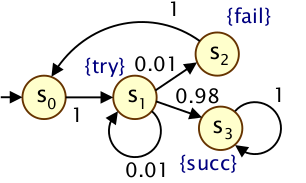
\includegraphics[scale=0.6]{DTMC.png} 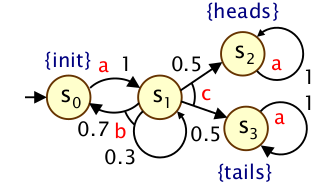
\includegraphics[scale=0.6]{MDP.png}
	\centering
	\caption{(a) DTMC \hspace{2cm} (b) MDP}
\end{figure}

\begin{figure}[h]
	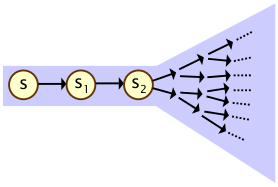
\includegraphics[scale=0.6]{cone.png}
	\centering
	\caption{Cilindro $C(w)$}
\end{figure}

Un camino, finito o infinito, a trav\'es de una DTMC, es una secuencia de estados $s_0s_1s_2...$ tales que $P(s_i, s_{i+1}) > 0$ $\forall i$, que representa una ejecuci\'on o comportamiento posible del sistema que el DTMC est\'a modelando. Para sacar conclusiones cuantitativas sobre este sistema es necesario definir un espacio de probabilidad sobre estos caminos. Los eventos que componen el espacio muestral $Path(s)$ ser\'an los conjuntos de caminos infinitos desde el estado $s$.  Dado un camino finito desde $s$, $w = ss_1s_2...s_n$, se definen los eventos b\'asicos denominados conjunto de cilindros (o conos) $C(w)$ al conjunto de los caminos infinitos con el prefijo com\'un $w$, como se ilustra en la Figura 2. La medida de probabilidad $Pr_s$ sobre el espacio muestral $Path(s)$, se define de la siguiente manera: $Pr_s(C(ss_1s_2...s_n)) = P(s,s_1)P(s_1,s_2)...P(s_{n-1}, s_n)$. As\'i por ejemplo: $Pr_s(C(ss_1s_2)) = P(s,s_1)P(s_1,s_2)$. \\

Pero, algunos aspectos de un sistema pueden no ser probabil\'isticos y por lo tanto no deben modelarse probabil\'isticamente; algunos casos posibles son:

\begin{itemize}
	\item Concurrencia y programaci\'on de componentes paralelos. Por ejemplo algoritmos distribuidos aleatorios o m\'ultiples procesos probabil\'isticos que operan asincr\'onicamente.
	
	\item Entornos desconocidos. Como en protocolos probabil\'isticos de seguridad. % o adversario desconocido.
	
	\item Subespecificaci\'on y par\'ametros del modelo desconocidos. Por ejemplo un protocolo de comunicaci\'on probabil\'istica dise\~nado para retrasos en la propagaci\'on de mensajes entre $d_{min}$ y $d_{max}$.
	
\end{itemize}

Para ello se definen los \textbf{Procesos de Decisi\'on de Markov (MDPs).} Estos son una extensi\'on de las DTMCs que permiten una elecci\'on no determinista. El conjunto de estados ser\'a discreto, las transiciones entre estados pasos de tiempo discretos, cuya elecci\'on es no determinista entre varias distribuciones discretas de probabilidad sobre estados sucesivos. En la Figura 1 (b) puede observarse un ejemplo de MDP.

Formalmente un MDP $M$ es una tupla $(S, s_0, Steps, L)$, donde $S$, $s_0$ y $L$ est\'an definidas igual que para las DTMCs, y $Steps: S \rightarrow 2^{Act \times  Dist(S)}$ es la funci\'on de transici\'on probabil\'istica donde $Act$ es un conjunto de acciones y $Dist(S)$ es el conjunto de las distribuciones de probabilidad discretas sobre el conjunto de estados $S$.

Un camino, finito o infinito, a trav\'es de un MDP es una secuencia de estados y pares de acci\'on / distribuci\'on $s_0(a_0, \mu_0)s_1 (a_1, \mu_1)s_2...$ donde $(a_i, \mu_i) \in Steps(s_i)$ y $\mu_i(s_{i+1})>0$. %notar que tanto la elecci\'on no determinista como la probabil\'istica se resuelven
Se define un adversario $A$, tambi\'en conocido como ``schedulers" o ``policies", como un mapeo desde cualquier camino finito en el MDP a un par de acci\'on / distribuci\'on posterior. Para un adversario $A$ el MDP se reduce a un DTMC (posiblemente con infinitos estados), el conjunto resultante de caminos infinitos es $Path^A(s)$, sobre el cual se puede definir una medida de probabilidad $Pr^A_s$. Entonces para razonar sobre el comportamiento probabil\'istico en un MDP, primero debe resolverse el no determinismo con un adversario. \\

Las \textbf{Cadenas de Markov de Tiempo Continuo (CTMCs)} son definidas de forma similar a las DTCM donde el espacio de estados es discreto, pero el tiempo es continuo y los retrasos (delays) est\'an distribuidos exponencialmente. Son adecuadas para modelos de vida \'util de componentes, tiempos entre llegadas, tasas de reacci\'on bioqu\'imica, etc. Tambi\'en se pueden definir los correspondientes MDPs de tiempo continuo. \\

%\textbf{Automata de Markov.} \\

Para la \textbf{especificaci\'on de propiedades} se puede utilizar, entre otras, PCTL (Probabilistic Computation Tree Logic) que es una l\'ogica temporal que extiende a la l\'ogica temporal no probabil\'istica CTL para poder describir propiedades cuantitativas de DTMCs/MDPs.

\section{Casos de estudio}

A continuaci\'on desarrollamos brevemente algunos casos de estudio m\'as importantes de la herramienta.
\paragraph{Automated Fine Tuning of Probabilistic Self-Stabilizing Algorithms. \cite{Saba}.}


Se trata de un proyecto conjunto de Canad\'a y Alemania, en el cual se estudiaron tres diferentes t\'ecnicas para encontrar la distribuci\'on de probabilidad que logr\'a el m\'inimo tiempo promedio de recuperaci\'on para un input de un protocolo randomizado, distribuido y autoestable sin que modifique el comportamiento del algoritmo. Una de las tres t\'ecnicas consist\'ia en usar Storm para la ``sintes\'is del par\'ametro", donde Storm computa la funci\'on racional, describiendo el tiempo promedio de recuperaci\'on y luego usa 'solvers' (solucionadores) para encontrar el par\'ametro \'optimo de valuaci\'on. Se evaluaron las t\'ecnicas con el algoritmo de 'Herman' (Randomized token circulation) y se obtuvo que la t\'ecnica que utilizaba Storm fue la segunda mas r\'apida.

\paragraph{odel-Checking Assisted Protocol Design for Ultra-Reliable Low-Latency Wireless Networks. \cite{Christian}}


Consiste en una t\'ecnica desarrollada en Suecia en conjunto con Alemania, para dise\~nar protocolos para aplicaciones de seguridad cr\'itica. Tradicionalmente el desarrollo de sistemas inal\'ambricos de baja latencia se bas\'o en simulaciones para identificar arquitecturas viables, la propuesta consisti\'o en usar Storm como herramienta de verificaci\'on probabil\'istica de modelos, para evaluar diferentes variantes de sistemas en la etapa de dise\~no. Se comprob\'o mediante el protocolo de EchoRing, pensado especialmente para aplicaciones industriales de seguridad cr\'itica y basado en sistemas de Tokens, que Storm es una potencial herramienta para la evaluaci\'on de los diferentes dise\~nos de mecanismos para el manejo de un token perdido.

\paragraph{Counterexamples for Expected Rewards.\cite{Tim}.}

Se trata de un estudio desarrollado en Alemania con el prop\'osito de demostrar que al emplear Storm como herramienta para la computaci\'on de contraejemplos en sistemas probabil\'isticos para ``recompezas esperadas o costos esperados", se puede obtener un subsistema minimial que ya lleva el costo o la recompenza m\'as alla del l\'imite permitido.

\paragraph{Bounded Model Checking for Probabilistic Programs. \cite{Nils}.}

Estados Unidos junto con Alemania investigaron la aplicaci\'on de los enfoques de la verificaci\'on estandar de modelos para verificar propiedades en programas probabil\'isticos. Como el modelo operacional de los programas probabil\'isticos estandar es un proceso potencial param\'etrico infinito de Markov, no es posible una adapctaci\'on directa a las t\'ecnicas existentes. Por lo tanto se propuso un enfoque intuitivamente donde el modelo operacional es creado exitosamente y verificado paso a paso mediante una ejecuci\'on del programa. La evaluaci\'on de dicho modelo es corroborado mediante benchmarks y utilizando Storm para la s\'intesis de par\'ametros.

\paragraph{Model-based Safety Analysis for Vehicle Guidance Systems.\cite{Majdi}.} 

Este caso de estudio es el que hemos elegido para exponer en mayor profundidad. Fue realizado en Alemania por los creadores de la herramienta en conjunto con la empresa automotriz BMW para el an\'alisis de 'safety' en la fase de dise\~no de los sistemas de direcci\'on asistida de los veh\'iculos.

El caso se dividio en 3 fases, Primero la construcci\'on de arboles din\'amicos de fallas apartir de la descripciones del sistema, Los sistemas varian segun la norma ISO 26262 donde 'safety-critically' es tecnicamente medido por lo que se llama ASIL (Automotive Safety Integrity Level), que va desde ASIL QM es ninguna medida de seguridad requerida hasta ASIL D (con ASIL A, B y C en el medio) que es el nivel de integridad de 'safety' mas alta. Luego combinar estos arboles din\'amicos de fallas de manera autom\'atica con modelos de fallas de hardware para diferentes partes funcionales de Hardware. Por \'ultimo  analizar los arboles din\'amicos de fallas con STORM.

Los arboles di\'namicos de fallas basicamente son estructuras que se crean a partir de arboles de fallas. Estos arboles son Grafos ac\'iclicos dirigidos con nodos tipados, los nodos son compuertas ('gates') y los nodos sin descendientes se llaman 'Eventos B\'asicos' ('BE'). Los arboles din\'amicos de fallas tienen mas funcionalidades, es decir mas tipos de compuertas, que permiten ser m\'as expresivos para definir el comportamiento del sistema cuando ocurre una falla.

El modelo basado en este caso de estudio se puede ver en la figura 3. Donde el comportamiento en caso de fallas de la arquitectura funcional, dado como 'functional block diagram' es expresado en un arbol din\'amico de fallas de 2 capas. La capa superficial modela al sistema de fallas en terminos de bloques de fallas $B_i$ mientras que la capa inferior modela las causas de las fallas de los bloques. Cada bloque funcional se le asigna una plataforma de Hardware donde un arbol din\'amico de fallas modela su comportamiento sobre las fallas.

\begin{figure}[h]
	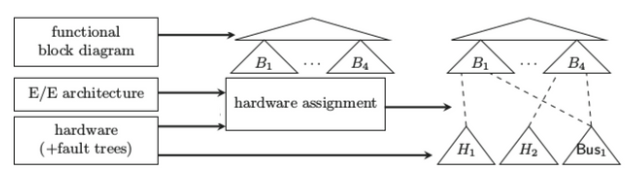
\includegraphics[scale=0.43]{modelbased.png} 
	\centering
	\caption{Modelo del caso de estudio en un enfoque de 'safety'}%Overview of the model-based safety approach
\end{figure}


Hay 4 enfoques para modelar los diagramas de bloques funcionales. Resumidamente, los diagramas funcionales cuentan con varios bloques, primero una cantidad de $s_i$ de sensores (camara del auto, sensores de proximidad, etc) que recolectan la informacion, luego un interpretador de la informacion recolectada, esa informacion es procesada por un Planeador de trayectorias que luego lo ejecutara el Administrador de actores con los actores $a_i$ (acelerador, freno, etc). No se va a profundizar en sus variantes pero difieren \'unicamente en como se comportan al momento de que una falla ocurra.
Lo importante es que cada variante de los diagramas de bloques funcionales definen una propiedad de safety diferente, para ello tambien se tuvo que implementar 3 formas distintas para los modelos de las arquitecturas E/E (el\'ectrico y electr\'onico). Pero en general, estos modelos comparten este mismo funcinonamiento. Dados los sensores $s_i$ existe un sistema avanzado de asistencia de conducir o varios que obtienen esa informaci\'on y las unidades de control el\'ectrico transfieren la informaci\'on mediante un Bus de datos a los actores $a_i$. Estos modelos del sistema varian segun los modelos previos de los diagramas de bloques, \'osea segun el comportamiento de los mismos a la hora de que ocurra una falla.

Al usar arboles din\'amicos de fallas para modelar este caso de estudio, fue muy fac\'il evaluarlo con Storm ya que se reescribi\'o los arboles de fallas en arboles din\'amicos de fallas con una t\'ecnica citada en \cite{Tree} y luego Storm traduce estos arboles en Automatas deterministas parametrizados de Markov y por \'ultimo son reducidos a cadenas de tiempo continuo de Markov. En este paso lo que queda es evaluar estas cadenas de Markov con unas propiedades de la herramienta (alcanzabilidad, alcanzabilidad en un tiempo limite sin haber estado en un estado malo, y tiempo esperado para alcanzar un estado dado). Como resultado se pudo obtener los resultados de las probabilidades de las fallas de los modelos, su Integridad bajo operaciones fallidas limitadas, Fallas a lo largo del tiempo y el analisis sensitivo. %(?)

%cita Junges, S., Guck, D., Katoen, J.P., Rensink, A., Stoelinga, M.: Fault trees on a diet: automated reduction by graph rewriting. Formal Asp. Comput. 29(4), 651–703 (2017)

\begin{figure}[h]
	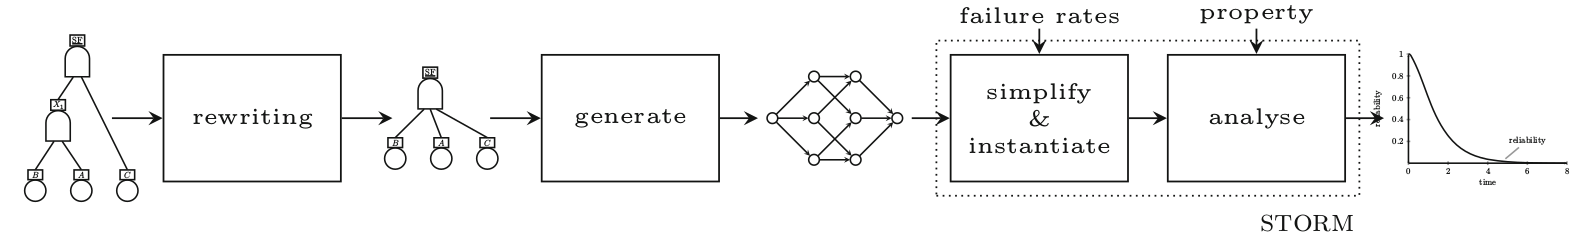
\includegraphics[scale=0.3]{stormapproach.png} 
	\centering
	\caption{Proceso de como storm evalu\'o el modelo}%Overview of the storm-dft approach
\end{figure}

Y en conclusi\'on se pud\'o demostrar que es posible usar arboles dinamicos de fallas para modelar este tipo de problemas y mostrar sus ventajas.




%donde  ayudan a definir el comportamiento del sistema.  Se propusieron dise~nar el modelo en tres capas de modelar los conceptos variados de seguridad y la arquitectura E/E (el\'ectrico y electr\'onico) para la conducci\'on automatizada: los \'arboles din\'amicos de fallas, los \'arboles de fallas y los \'arboles est\'aticos de fallas. La mejor forma result\'o ser usar los \'arboles din\'amicos de fallas, la mayor ventaja es que, adem\'as de ser m\'as expresivos que un \'arbol est\'atico, se pueden analizar por medio de Storm.

%En la Figura 3 se observan los Diagramas de bloques de la direcci\'on del veh\'iculo, hay cuatro diagramas posibles (a), (b), (c) y (d). $s_i$ representa los sensores del veh\'iculo, $EP$ (Enviroment Perceptor) percibe toda la informaci\'on de los sensores, $TP$ (Trayectory Planning) crea una nueva trayectoria de acuerdo a la informaci\'on recibida, $AM$ (Actuator Management) env\'ia la informaci\'on sobre las nuevas acciones a ejectutar. Los $a_i$ representan a los actores. En el caso del diagrama (b) $Voter$ elige la trayectoria m\'as segura antes de transmitirla a los actores. En el diagrama (c) $TCS$ (Trajectory Checking and Selection) elige la trayectoria mas segura en caso de haber una falla. Por \'ultimo, en el diagrama (d) $Switch$ elige los componentes $fb$-$EP$ y $fb$-$TP$ para le percepci\'on de la informaci\'on y el planeamiento de la trayectoria ya que son los componentes de back-up en caso de una falla.

%\begin{figure}[h]
%	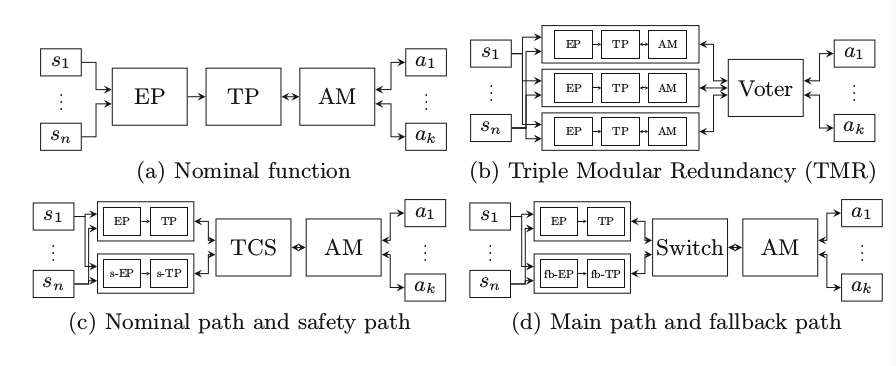
\includegraphics[scale=0.43]{blockdiagram.png} 
%	\centering
%	\caption{Diagramas de bloques de la direcci\'on del veh\'iculo}
%\end{figure}

%En la Figura 4 se ilustran los diferentes modelos de arquitecturas E/E, $ADAS$ (Advanced Driver Assistance System) es una plataforma conectada a todos los sensores donde esta implementada la funci\'on de dirrecci\'on del veh\'iculo, $ECU$ (Electronic Control Unit) son las las unidades de control de los actores y en caso de $I-ECU$ (Integration ECU) donde funciones no dedicadas pueden ser implementadas.

%\begin{figure}[h]
%	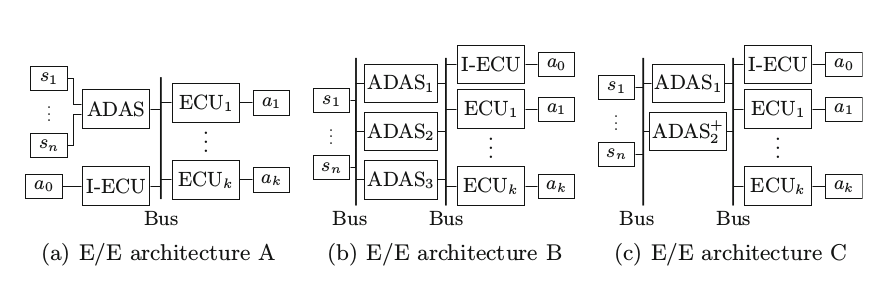
\includegraphics[scale=0.4]{EE.png}
%	\centering
%	\caption{Diferentes modelos de arquitecturas E/E}
%\end{figure}

%Storm puede convertir los \'arboles din\'amicos de fallas a un Automata de Markov (parametrizado y determinista) y luego reducir el aut\'omata a una cadena param\'etrica de tiempo continuo de Markov.

%Entonces se modelaron cuatro diferentes diagramas de bloques para la direcci\'on de los veh\'iculos con sus respectivos \'arboles de fallas y tres diferentes arquitecturas E/E, que se diferenciaban en las decisiones que tomaban luego de que una falla ocurriera y se combinan para los distintos conceptos de 'safety', creando ocho diferentes \'arboles din\'amicos de fallas, que se chequearon con Storm obteniendo los siguientes resultados en las correspondientes propiedades de safety:

%\begin{itemize}
%	\item $FIT$: Failures in time,
%	\item $SILFO$: System Integrity under Limited Fail-Operation,
%	\item $Sentivity$ $analysis$ y $Probability$ $of$ $failure$
%\end{itemize}

%dando como resultado los siguientes gr\'aficos y demostrando el el modelo SC2/B resulto ser el mejor. (Combinacion Figura 3.b) y Figura 4.2))	

%En la Figura 5 se observan los resultados, los mismos demuestran que el modelo SC2/B result\'o ser el mejor, como puede deducirse al combinar las Figuras 3(b) y 4(b). 

%\begin{figure}[h]
%	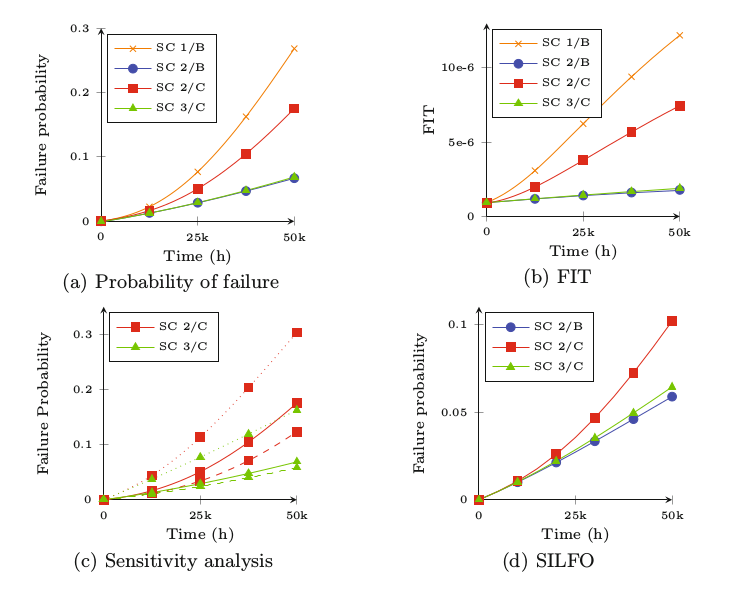
\includegraphics[scale=0.5]{results.png}
%	\centering
%	\caption{Resultados}
%\end{figure}


\section{Comparaci\'on con otras herramientas.}

Otros model checkers probabil\'isticos: PRISM (utiliza DTMCs, MDPs, CTMCs), ETMCC/MRMC (utiliza DTMCs, CTMCs), LiQuor (verificaci\'on LTL para MDPs), RAPTURE (prototipo para la abstracci\'on / refinamiento de MDPs). Model checkers probabil\'isticos basados en simulaci\'on: APMC, Ymer, VESTA; de comprobaci\'on de CSL para CTMCs: APNN-Toolbox, SMART; para m\'ultiples formalismos: CADP, M\"{o}bius.

\section{Conclusiones.}

\begin{thebibliography}{99}
	\bibitem{Saba} Saba Aflaki, Matthias Volk, Borzoo Bonakdarpour, Joost-Pieter Katoen, Arne Storjohann. Automated Fine Tuning of Probabilistic Self-Stabilizing Algorithms. Proc. of 36th IEEE Symposium on Reliable Distributed Systems (SRDS), pages 94–103, IEEE CS (Recipient of Best Paper Award), 2017.	
		
	\bibitem{Christian} Christian Dombrowski, Sebastian Junges, Joost-Pieter Katoen, James Gross. Model-Checking Assisted Protocol Design for Ultra-Reliable Low-Latency Wireless Networks. Proc. of the 35th Symp. on Reliable Distributed Systems (SRDS), pages 307–316, IEEE CS, 2016.
	
	\bibitem{Tim} Tim Quatmann, Nils Jansen, Christian Dehnert, Ralf Wimmer, Erika Abraham, Joost-Pieter Katoen, Bernd Becker. Counterexamples for Expected Rewards. Proc. of the 20th Int. Symp. on Formal Methods (FM'15), Volume 9109 of LNCS, pages 435–452, Springer, 2015.
	
	\bibitem{Nils} Nils Jansen, Christian Dehnert, Benjamin Lucien Kaminski, Joost-Pieter Katoen, Lukas Westhofen. Bounded Model Checking for Probabilistic Programs. Proc. of the 14th International Symposium on Automated Technology for Verification and Analysis (ATVA 2016), Volume 9938 of LNCS, Springer, 2016.
	
	\bibitem{Majdi} Majdi Ghadhab, Sebastian Junges, Joost-Pieter Katoen, Matthias Kuntz, Matthias Volk. Model-based Safety Analysis for Vehicle Guidance Systems. Proc. of SAFECOMP, Volume 10488 of LNCS, pages 3–19, Springer, 2017.
	
	\bibitem{Tree} Junges, S., Guck, D., Katoen, J.P., Rensink, A., Stoelinga, M.: Fault trees on a diet: automated reduction by graph rewriting. Formal Asp. Comput. 29(4), 651–703 (2017)

\end{thebibliography}


\end{document}
